\chapter{Analisis Requerimientos y Riesgos}
	
	\section{Introducción}
	\par
	Como primera acción se analizó la factibilidad de implementación de un SoC con licencia OpenSource en FPGA, razón que condujo a la investigación del
	tópico en búsqueda de información necesaria que determine si existe tal posibilidad. Las características relevadas durante la investigación
	aportaron información respecto al hardware, las herramientas de desarrollo y el sistema operativo necesario para llevar a cabo la implementación. 
	\vspace{0.5cm}
	\par
	Para la selección del SoC se debió definir el microprocesador y los periféricos a utilizar, como así también las herramientas necesarias para la
	compilación y depuración de aplicaciones que corran sobre él. Esta situación derivó en una valoración de los diferentes entornos de desarrollo y
	sistemas operativos asociados que cumplan con el paradigma del software libre. Fue necesario además discernir entre las diversas alternativas de
	hardware que se tenían disponibles al momento del desarrollo de este trabajo compatibles con el SoC seleccionado. 
	\vspace{0.5cm}
	\par
	Fue necesario evaluar la posibilidad de implementar un Sistema Operativo que provea acceso mediante drivers a todos los periféricos conectados a
	la plataforma hardware elegida. La síntesis e implementación sobre FPGA requiere de aplicaciones específicas que debieron ponderarse para alcanzar el
	cumplimiento de los requerimientos.
	
	\newpage 
	
	\section{Requerimientos del Usuario}
	\par
	Se presenta en este apartado un listado de los requerimientos elecitados que tienen como objetivo comprender el dominio del problema y permiten
	trabajar en la realización de una solución eficiente.
	
		\subsection{En cuanto al hardware}
		\begin{table}[h]
		\centering
		\begin{tabular}{ p{2.5cm} p{8cm} p{3cm} }
		\hline 
		\rowcolor[gray]{0.8} N\textordmasculine Req & Descripción & Tipo\\
		\hline
		RQX-HW 1 &  Se debe implementar un Microprocesador Softcore de núcleo simple & Cantidad y tipo de núcleos. \\
		\hline
		RQX-HW 2 &  El SoC seleccionado debe poseer la menor cantidad de restricciones respecto de su implementación en placas de desarrollo de diversos
		fabricantes. & Portabilidad a nivel Hardware\\
		\hline
		RQX-HW 3 & La placa de desarrollo elegida debe poseer al menos 32 MB de memoria RAM disponible que permita al ejecución del kernel de linux. &
		Memoria Disponible\\
		\hline
		RQX-HW 4 & La placa de desarrollo elegida debe poseer al menos 8 MB de memoria flash disponible que permita guardar la configuración de la FPGA y un
		bootloader & Memoria Disponible\\
		\hline
		\end{tabular}
		\caption{Listado de requerimientos de usuario - Hardware}
		\label{tab:requsr1}
		\end{table}
					
		\subsection{En cuanto a las licencias}
		\begin{table}[h]
		\centering
		\begin{tabular}{ p{2.5cm} p{8cm} p{3cm} }
		\hline 
		\rowcolor[gray]{0.8} N\textordmasculine Req & Descripción  & Tipo\\
		\hline 
		RQX-LC 1 &  Todo el codigo RTL implementado debe tener licencia LGPL o GPL en su defecto & Licencias de hardware\\
		\hline 
		RQX-LC 2 &  Las herramientas de desarrollo utilizadas para el diseño de hardware  deben poseer licencias LGPL o GPL en su defecto & Licencias de Software\\
		\hline 
		RQX-LC 3 &  Las herramientas de desarrollo de saoftware utilizadas para deben poseer licencias LGPL o GPL en su defecto & Licencias de Software\\
		\hline
		RQX-LC 4 & El sistema operativo elegido debe poseer licencia LGPL o GPL & Licencias de Software\\
		\hline
		\end{tabular}
		\caption{Listado de requerimientos de usuario - Licencias}
		\label{tab:requsr2}
		\end{table}
		
		\newpage
			
		\subsection{En cuanto a las herramientas de desarrollo}
		\begin{table}[h]
		\centering
		\begin{tabular}{ p{2.5cm} p{8cm} p{3cm} }
		\hline 
		\rowcolor[gray]{0.8} N\textordmasculine Req & Descripción  & Tipo\\
		\hline 
		RQX-HD 1 &  Las herramientas de desarrollo de Software y Hardware deben tener la menor cantidad de restricciones respecto del sistema operativo donde serán ejecutadas & Portabilidad\\
		\hline 
		RQX-HD 2 &  Las herramientas de desarrollo de Software deben brindar la capacidad de compilar y depurar programas para la arquitectura seleccionada &
		Herramientas de Software\\
		\hline
		RQX-HD 3 &  Las herramientas de desarrollo de Hardware para la placa seleccionada deben proveer soporte para el acceso a sus periféricos on board &
		Herramientas de Hardware\\ 
		\hline 
		\end{tabular}
		\caption{Listado de requerimientos de usuario - Herramientas de desarrollo}
		\label{tab:requsr3}
		\end{table}
		
		\subsection{En cuanto sistema operativo} 	 
		\begin{table}[h]
		\centering
		\begin{tabular}{ p{2.5cm} p{8cm} p{3cm} }
		\hline 
		\rowcolor[gray]{0.8} N\textordmasculine Req & Descripción  & Tipo\\
		\hline 
		RQX-SO 1 &  El sistema operativo elegido debe disponer de drivers y librerías que permitan el acceso a todos los dispositivos incluídos en el SoC &
		Driver y Librerías\\
		\hline 
		RQX-SO 2 &  El sistema operativo elegido debe tener la capacidad de ejecución multitarea e hilos & capacidad de ejecución del SO\\ 
		\hline
		RQX-SO 3 &  El sistema operativo elegido debe posibilitar la ejecución de aplicaciones de tiempo real & Sistema Operativo\\ 
		\hline 
		\end{tabular}
		\caption{Listado de requerimientos de usuario - Sistema operativo}
		\label{tab:requsr4}
		\end{table}
	
	\newpage
	
	\section{Análisis de Riesgo}
		\subsection{Introducción}
        Para lograr producir aquello que se requiere, en el plazo solicitado y ajustados al presupuesto asignado, se necesita desarrollar
        un proceso que incluya desde la etapa más temprana la gestión de los riesgos asociados a los requerimientos, de forma que se contribuya al
        mejoramiento gradual del proceso de desarrollo y la gestión de un proyecto.
		\vspace{0.5cm}
		\par
        La gestión de riesgos procura formalizar conocimiento orientado a la minimización de riesgos en proyectos, mediante la
        generación de principios y buenas prácticas de aplicación realista \cite{etiqueta_riegos1}. Hasta el momento se ha propuesto
        y utilizado diferentes enfoques de gestión del riesgo desde que Boehm \cite{etiqueta_riegos2} atrajo a la comunidad de ingeniería del
        software hacia la gestión del riesgo. Sin embargo, es evidente que pocas organizaciones utilizan todavía de una forma explícita y sistemática
        métodos específicos para gestionar los riesgos en sus proyectos.
		\vspace{0.5cm}
		\par
        En \cite{etiqueta_riegos3} se presenta la definición de riesgo que plantea que el riesgo afecta a los futuros acontecimientos, implica
        cambios, e implica elección conjunto a la incertidumbre asociada a la misma. Es indiscutible que están presentes permanentemente las características de
        incertidumbre (acontecimiento que caracteriza al riesgo y que puede o no ocurrir) y de pérdida (si el riesgo se convierte en una realidad
        ocurrirán consecuencias no deseables o pérdidas).
		\vspace{0.5cm}
		\par
		Están definidas las categorías de riesgos: los riesgos del proyecto, que amenazan el plan; los riesgos técnicos, que amenazan la calidad y la
		planificación temporal; y los riesgos del negocio, que amenazan la viabilidad del proyecto o del producto. Otra categorización a considerar a
		partir del conocimiento que se tenga de ellos: los riesgos conocidos (los que se descubren en las evaluaciones); los riesgos predecibles (se
		extrapolan de la experiencia) y los riesgos impredecibles (pueden ocurrir, pero es muy difícil identificarlos de antemano).
		\vspace{0.5cm}
		\par
     	También son claras las estrategias frente al riesgo. Por un lado están las reactivas, cuyo método es evaluar las consecuencias del riesgo cuando
 		este ya se ha producido (ya no es un riesgo) y actuar en consecuencia. Este tipo de estrategias acarrea consecuencias negativas, al poner el
 		proyecto en peligro. Y por el otro las proactivas, que aplican el método de evaluación previa y sistemática de los riesgos y sus posibles
 		consecuencias, a la par que conforman planes de contingencias para de evitar y minimizar las consecuencias. Consecuentemente, este tipo de
 		estrategias permite lograr un menor tiempo de reacción ante la aparición de riesgos impredecibles.
		\vspace{0.5cm}
		\par
		De acuerdo con \cite{etiqueta_riegos3}, la administración o gestión de riesgos es un proceso iterativo que se aplica durante todo el proyecto y se
		desarrolla en cuatro etapas detalladas en la Figura ~\ref{fig:riesgos}. Se utilizó este modelo como guía para el análisis de los riegos del
		proyecto.
		
		\begin{figure}[!h]
 		\begin{center}
  		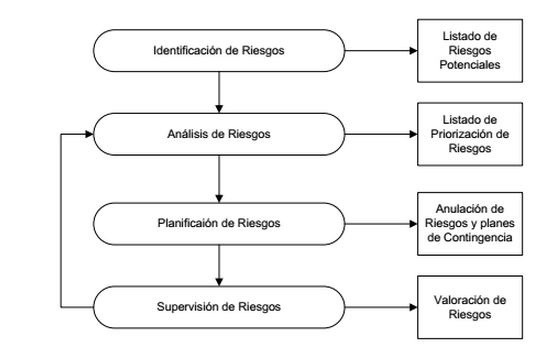
\includegraphics[width=0.8\textwidth,keepaspectratio=true]{./images/riesgos}
  		\caption{Procedimiento para la gestión de riesgos}
  		\label{fig:riesgos}
 		\end{center}
		\end{figure}
		
		\subsection{Identificación y análisis de riesgos}
		\par
		Se realizó un relevamiento inicial de riegos respecto de cada requerimiento de usuario planteado. Fue efectuado un análisis de severidad y
		probabilidad de ocurrencia para cada riesgo asociado. La severidad	del	impacto	de un riesgo concretado	se medió de la siguiente
		manera:
		
		\begin{itemize}
		  \item Catastrófico
		  \item Crítico	
		  \item Severo	
		  \item Menor	
		  \item Despreciable 
		\end{itemize}
	
		La probabilidad de ocurrencia se midió en base a la siguiente categorización:
	
		\begin{itemize}
		  \item Muy Probable
		  \item Probable	
		  \item Ocasional
		  \item Improbable 	
		  \item Remoto
		\end{itemize}
		
		En la Tabla ~\ref {tab:riegos} se listan los riesgos asociados, su severidad y probabilidad de ocurrencia para cada uno de los
		requerimientos de usuario.
		
		\newpage
		
		\begin{table}[!h]
		\centering
		\begin{tabular}{ p{2.5cm} p{9cm} p{2cm} p{2cm} }
		\hline 
		\rowcolor[gray]{0.8} N\textordmasculine Req & Riegos Asociados & Severidad  & Ocurrencia \\
		\hline
		RQX-HW 1& Código RTL con fallas reconocidas durante el proceso de síntesis & Crítica       & Probable \\
		\hline
				& Capacidad insuficiente para implementar la lógica del proyecto   & Catastrófico  & Ocasional\\	 
		\hline
		RQX-HW 2& Imposibilidad de acceso a alguno de los periféricos de la placa de desarrollo &  Crítica  & Probable\\
		\hline
		RQX-HW 3& Limitaciones de memoria RAM en las placas de desarrollo disponibles 	& Crítico  &  Improbable\\	 
		\hline
		RQX-HW 4& Limitaciones de memoria FLASH en las placas de desarrollo disponibles & Severo  &  Improbable\\ 
		\hline
		RQX-LC 1& Inexistencia de los Cores Open Source necesarios  	& Catastrófico  &  Ocasional\\
		\hline
				& Falta de documentación de apoyo para la implentación de los Cores  & Severo  &  Muy Probable\\ 
		\hline
		 		& Código RTL con fallas reconocidas durante el proceso de síntesis   & Critica & Probable\\ 
		\hline
		RQX-LC 2& Inexistencia de herramientas de desarrollo de hardware con licencias Open Source & Severo  &  Probable\\
		\hline
		RQX-LC 3& Inexistencia de herramientas de desarrollo de software con licencias Open Source & Severo  &  Improbable\\
		\hline
		RQX-LC 4& Inexistencia de un sistema operativo embebido con licencia Open Source  & Critico  &  Improbable\\
		
		\hline
		RQX-HD 1& Falta de herramientas de desarrollo portables a diversos sistemas operativos & Severo  &  Ocasional\\
		\hline		
		RQX-HD 2& Compilación cruzada incompatible con la arquitectura destino  & Critico &  Ocasional\\
		\hline
				& Falta de mecanismos de optimización de código del compilador  & Severo  &  Probable\\
		\hline
				& Imposibilidad de depuración de programas en la arquitectura destino& Crítico  &  Probable\\
		\hline
		RQX-HD 3& Soporte de acceso a periféricos inexistente o con presencia de bugs & Critico &  Probable\\
		\hline
		RQX-SO 1& Drivers necesarios inexistentes o con fallos & Critico &  Probable\\
		\hline
				& Librerías necesarias inexistentes o con fallos & Severo &  Probable\\
		\hline
		RQX-SO 2& Incapacidad de ejecución de hilos en los SO compatibles con el microprocesador elegido & Catastróficos & Improbable\\
		\hline
		RQX-SO 3& Limitaciones para la ejecución de SO de tiempo real & Critico & Probable\\
		\hline
		\end{tabular}
		\caption{Tabla de riegos vs. Requerimientos}
		\label{tab:riegos}
		\end{table}
	
		\newpage
		\subsection{Planificación de los riesgos}	

Se presentan a continuación en la Tabla ~\ref {tab:planificación} las estrategias para reducir o eliminar el impacto de los riesgos detectados y analizados anteriormente. Estas estrategias generarán requerimientos de confiabilidad del sistema debido a que definen una defensa frente al riesgo y cómo este se gestionará en caso de ocurrir.
	
        \begin{table}[!h]
		\centering
		\begin{tabular}{ p{4cm} p{4cm} p{4cm} p{3cm} }
		\hline 
		\rowcolor[gray]{0.8} Riesgo & Consecuencia & Estrategia preventiva & Estrategia de contingencia\\
		\hline
		Código RTL con fallas reconocidas durante el proceso de síntesis& Retraso en los tiempos de implementación & Análisis previo de guías de resolución de problemas y preguntas frecuentes & Revisión de código y consulta a los desarrolladores \\
		\hline
		 Capacidad insuficiente para implementar la lógica del proyecto & Imposibilidad de implementación en el hardware disponible  & Verificación de datos de espacio lógico necesario  & Cambio de kit de desarrollo\\	 
		\hline
		 Imposibilidad de acceso a alguno de los periféricos de la placa de desarrollo & Imposibilitad de implementar cualquier diseño de Hardware que involucren esos periféricos& Verificar previamente e individualmente el funcionamiento de los periféricos & Cambiar el kit de desarrollo\\
		\hline
		Limitaciones de memoria RAM en las placas de desarrollo disponibles& Imposibilidad de ejecución de las aplicaciones requeridas & Verificación previa de los recursos utilizados por las aplicaciones a ejecutar & Adición de un nuevo módulo al código RTL  \\	 
		\hline
		Limitaciones de memoria FLASH en las placas de desarrollo disponibles& Incapacidad de disponer en memoria no volátil de una aplicación de arranque (bootloader) & Verificación previa del espacio necesario para la aplicación de arranque & Búsqueda de un modo alternativo de arranque\\ 
		\hline
		Inexistencia de los Cores Open Source necesarios& Perdida de tiempo y dinero en la búsqueda de nuevo hardaware& Analisis previo de los cores Open Source existentes & Adquisición de IP cores\\
		\hline
		Falta de documentación de apoyo para la implentación de los Cores & Perdida de tiempo en realizar la implementación de los componentes & Revisión previa de la documentación existente para la elección de los  componentes & Dedicación de mayor tiempo para la implementación\\ 
		\hline
		 Inexistencia de herramientas de desarrollo de hardware con licencias Open Source & Imposibilidad de diseñar e implementar el Hardware & Verificar previamente la existencia de herramientas libres & Utilización de herramientas privativas con costos\\
		\hline
		\end{tabular}
		\end{table}
		\newpage
		\begin{table}[!h]
		\centering
		\begin{tabular}{ p{4cm} p{4cm} p{4cm} p{3cm} }
		\hline 
		\rowcolor[gray]{0.8} Riesgo & Consecuencia & Estrategia preventiva & Estrategia de contingencia\\
		\hline
		Inexistencia de herramientas de desarrollo de software con licencias Open Source & Imposibilidad de compilación y depuración de aplicaciones &Comprobación de la existencia de herramientas libres & Desarrollo de las herramientas necesarias\\
		\hline
		Inexistencia de un sistema operativo embebido con licencia Open Source  & Ejecución única de aplicaciones bare metal  & Análisis previo de los sistemas operativos embebidos disponibles & Desarrollo de las aplicaciones necesarias que fueran provistas por el SO\\
		\hline		
		 Falta de herramientas de desarrollo portables a diversos sistemas operativos & Imposibilidad de desarrollo de aplicaciones& Verificar la posibilidad de ejecución de las herramientas en diferentes SO& Utilización de las herramientas en alguno de los SO compatibles\\
		\hline		
		 Compilación cruzada incompatible con la arquitectura destino& Imposibilidad de ejecución de las aplicaciones desarrolladas & Analizar la compatibilidad previa a la elección del SO &  Verificación y depuración del código de la herramienta de complilación cruzada. \\
		\hline
		Falta de mecanismos de optimización de espacio de código por parte del  compilador&Exceso de tamaño de los binarios generados & Análisis previo de los compiladores disponibles & Implementación del core de memoria necesario\\
		\hline
		Imposibilidad de depuración de programas en la arquitectura destino& Imposibilidad de ejecución paso a paso y eliminación de errores &Prueba del depurador con simulador de arquitectura & Revisión del código del depurador \\
		\hline
		Soporte de acceso a periféricos inexistente o con presencia de bugs & Imposibilidad de desarrollar soluciones que involucren el uso de estos periféricos & Verificación individual de las herramientas que proveen el acceso a estos periféricos & Búsqueda  de  aplicaciones alternativa o desarrollo de las mismas\\
		\hline
		 Drivers necesarios inexistentes o con fallos & Imposibilidad de utilización de los dispositivos necesarios&Análisis previo de los driver de los dispositivos a utilizar &  Desarrollo de los drivers necesarios\\
		\hline
		Librerías necesarias inexistentes o con fallos& Imposibilidad de ejecución de aplicaciones sobre el sistema operativo embebido elegido & Análisis previo de las librerías disponibles y revisión de posibles bugs informados &  Desarrollo de las librerías necesarias o corrección de errores\\
		\hline
		\end{tabular}
		\end{table}
		\newpage
		\begin{table}[!h]
		\centering
		\begin{tabular}{ p{4cm} p{4cm} p{4cm} p{3cm} }
		\hline 
		\rowcolor[gray]{0.8} Riesgo & Consecuencia & Estrategia preventiva & Estrategia de contingencia\\
		\hline
		Incapacidad de ejecución de hilos en los SO compatibles con el microprocesador elegido &  Imposibilidad de ejecución para aplicaciones multitarea y/o multihilo & Análisis de los SO que cumplan con este requerimiento & Modificación del SO para el cumplimiento de las capacidades necesarias\\
		\hline
		Limitaciones para la ejecución de SO de tiempo real& Inviabilidad para la ejecución de aplicaciones en tiempo real & Análisis de los RTOS & Modificación del SO  para el cumplimiento de las capacidades de ejecución en tiempo real \\
		\hline
		\end{tabular}
		\caption{Planificación de riesgos}
		\label{tab:planificación}
		\end{table}
		
	